\section{Кривые}
\subsection{Классификация замкнутых регулярных кривых на плоскости с точностью до регулярной гомотопии}

\begin{definition}
    \textit{Непрерывная кривая} — непрерывное отображение отрезка в плоскость: $$\gamma: [a,b] \to \R^2.$$
    $$\gamma: (x(t), y(t))$$ — параметрическая кривая ($t$ — параметр).
\end{definition} 

\begin{definition}
    \textit{Гладкая параметрическая кривая} $\gamma = (x(t), y(t))$, $\gamma: [a,b] \to \R^2$, где $x(t), y(t) \in C^{\infty}([a,b])$. То есть, гладкая параметрическая кривая — это кривая, которая должна задаваться гладкими функциями, если записать её в координатах.
\end{definition}

В нашем курсе мы рассматриваем параметрические кривые, поэтому кривые, которые задаются, например, следующими параметрами:
$$\begin{cases}
    x = \cos{t}, \\
    y = \sin{t}, \\
    t \in [0, 2 \pi].
\end{cases}
\begin{cases}
    x = \cos{2t}, \\
    y = \sin{2t}, \\
    t \in [0, 2 \pi].
\end{cases}$$
разные, хотя как множество точек на плоскости они одинаковые.

Есть два подхода определения гладкой кривой:
\begin{enumerate}
    \item Образ кривой должен выглядеть как гладкая линия;
    \item Кривая, если её записать в координатах, должна задаваться гладкими функциями.
\end{enumerate}

\begin{example}
    Рассмотрим негладкую кривую, которая задаётся гладкими функциями (см.рис.\ref{fig:c12.1}).
    \begin{figure}[ht]
        \centering
        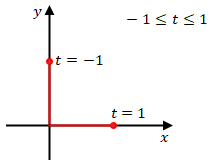
\includegraphics[scale=0.7]{images/c12.1.png}
        \caption{Негладкая линия, задаваемая гладкими функциями.}
        \label{fig:c12.1}
    \end{figure}

    Данная кривая задаётся следующими гладкими функциями (их графики см. на рис.\ref{fig:c12.2}):
    \[x(t) = \begin{cases}
        0,\ t \in [-1,0] \\
        e^{-\frac{1}{t}},\ t \in (0,1]
    \end{cases}
    y(t) = \begin{cases}
        e^{\frac{1}{t}},\ t \in [-1,0) \\
        0,\ t \in [0,1]
    \end{cases}
    \]

    \begin{figure}[ht]
        \centering
        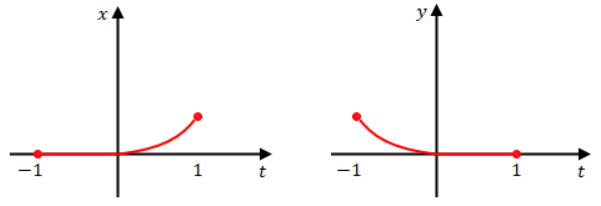
\includegraphics[scale=0.5]{images/c12.2.png}
        \caption{Графики гладких функций.}
        \label{fig:c12.2}
    \end{figure}
\end{example}

\begin{example}
    Наоборот, рассмотрим кривую, график которой выглядит гладким, но которая задаётся негладкими функциями (см.рис.\ref{fig:c12.3}).
    \begin{figure}[ht]
        \centering
        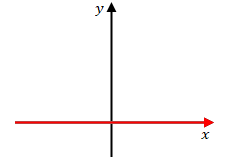
\includegraphics[scale=0.7]{images/c12.3.png}
        \caption{Гладкая линия, задаваемая негладкими функциями.}
        \label{fig:c12.3}
    \end{figure}
    Прямую $y = 0$ можно задать негладкими функциями, например:
    \[x(t) = |t| + t,\]
    \[y(t) = 0.\]
\end{example}

Чтобы объединить два данных подхода, определим понятие регулярной кривой.

\begin{definition}
    \textit{Регулярная кривая} — гладкая параметрическая кривая $\gamma(t) = (x(t), y(t))$, для которой вектор $\gamma'(t) = (x'(t), y'(t))$ (вектор скорости кривой) всюду отличен от нуля.
\end{definition}

\begin{definition}
    Для гладкой кривой $\gamma: [a,b] \to \R^2$ её \textit{вектором скорости в точке $t_0 \in [a,b]$} называется вектор 
    \[\frac{d\gamma}{dt}\Big|_{t=t_0} = \left(\frac{dx}{dt}\Big|_{t=t_0}, \frac{dy}{dt}\Big|_{t=t_0}\right).\]
\end{definition}

\begin{remark}
    Если кривая регулярная. то она в окрестности каждой своей точки будет выглядеть как гладкая линия (то есть, представима как график гладкой функции).
\end{remark}

\begin{definition}
    Пусть $\gamma(t) = (x(t), y(t))$, а $x(t), y(t)$ — гладкие периодические функции с периодом $T$. Тогда $\gamma: \R \to \R^2$ — \textit{гладкая замкнутая кривая}.
\end{definition} 

\begin{remark}
    Чтобы не нарушалась гладкость кривой, можно потребовать, чтобы векторы скорости в начальной и конечной точке совпадали, а можно считать, что функции $x(t), y(t)$ заданы не на отрезке, а на всей числовой прямой (как периодические функции) — в этом случае нам неважно, какая из точек отрезка $[a,b]$ выбрана за начальную или конечную.
\end{remark}

\begin{definition}
    Две замкнутые гладкие регулярные кривые $$\gamma_0(t), \gamma_1(t): \ [0, T] \to \R^2$$ называются \textit{регулярно гомотопными}, если существует отображение $$\gamma(t,s): [0, T] \times [0,1] \to \R^2,$$ которое:
    \begin{enumerate}
        \item является гладким;
        \item $s = 0, \ \gamma(t,s) \equiv \gamma_0(t); \ s = 1,\ \gamma(t,s) \equiv \gamma_1(t)$;
        \item $\gamma(t,s)$ при фиксированном $s$ — гладкая замкнутая регулярная кривая.
    \end{enumerate}
\end{definition} 

\begin{figure}[ht]
    \centering
    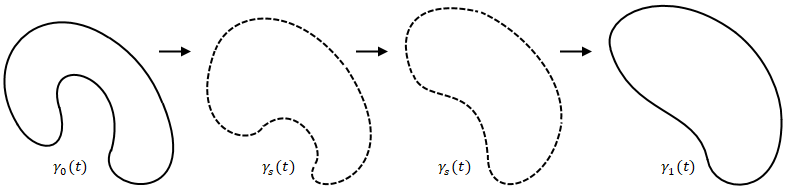
\includegraphics[scale=0.5]{images/c12.4.png}
    \caption{Регулярно гомотопные кривые.}
    \label{fig:c12.4}
\end{figure}

\begin{definition}
    Две замкнутые непрерывные кривые $$\gamma_0(t), \gamma_1(t): \ [0, T] \to \R^2$$ называются \textit{гомотопными}, если существует отображение $$\gamma(t,s): [0, T] \times [0,1] \to \R^2,$$ которое:
    \begin{enumerate}
        \item является непрерывным;
        \item $s = 0, \ \gamma(t,s) \equiv \gamma_0(t); \ s = 1,\ \gamma(t,s) \equiv \gamma_1(t)$;
        \item $\gamma(t,s)$ при фиксированном $s$ — непрерывная замкнутая кривая.
    \end{enumerate}
\end{definition} 

\begin{definition}
    Две гладкие регулярные кривые $$\gamma_0(t), \gamma_1(t): \ [0, T] \to \R^2$$ называются \textit{регулярно гомотопными}, если существует отображение $$\gamma(t,s): [0, T] \times [0,1] \to \R^2,$$ которое:
    \begin{enumerate}
        \item является гладким;
        \item $s = 0, \ \gamma(t,s) \equiv \gamma_0(t); \ s = 1,\ \gamma(t,s) \equiv \gamma_1(t)$;
        \item $\gamma(t,s)$ при фиксированном $s$ — гладкая регулярная кривая.
    \end{enumerate}
\end{definition} 


Пусть $\gamma$ — гладкая регулярная кривая такая, что $$\gamma: [0, T] \to \R^2,\ (x(t), y(t)),$$ $$\bar{0} \neq v = (x'(t), y'(t)) = (\rho(t) \cos{\phi(t)}, \rho(t) \sin{\phi(t)}),$$ где $\rho(t) > 0$ (длина $v$).

\begin{definition}
    \textit{Число вращения для замкнутой регулярной кривой $\gamma$} — число $$R(\gamma) = \frac{\phi(T) - \phi(0)}{2 \pi} \in \Z$$
\end{definition}

\begin{remark}
    Число вращения — это число оборотов, которое совершит вектор скорости при движении точки от начала до конца кривой.
    Например, для кривой на рис.\ref{fig:c12.5} $R(\gamma) = 1$.
    \begin{figure}[htbp]
        \centering
        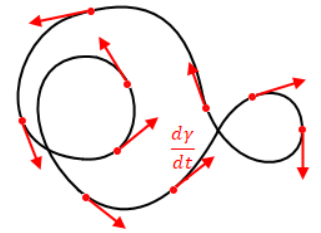
\includegraphics[scale=0.7]{images/c12.5.png}
        \caption{Вычисление числа вращения.}
        \label{fig:c12.5}
    \end{figure}
\end{remark}

\begin{remark}
    Число вращения — инвариант, отвечающий за регулярную гомотопность кривых.
\end{remark}

\begin{theorem}[Уитни]
    Две гладкие замкнутые регулярные кривые на плоскости регулярно гомотопны тогда и только тогда, когда их числа вращения совпадают.
\end{theorem}

Например, окружность с петлёй нельзя продеформировать в окружность, потому что их числа вращений не совпадают.

Пусть $\gamma(t)$ — гладкая регулярная кривая. $\gamma'(t) = (x'(t), y'(t))$ — ненулевой вектор скорости.

\begin{definition}
    Гладкая регулярная кривая называется \textit{натурально параметризуемой кривой}, если длина её вектора скорости равна 1.
\end{definition} 

% \begin{statement}
%     Для любой гладкой регулярной кривой существует натуральная параметризация $\gamma(t)$.
% \end{statement} 

% $$S = \int_{0}^{t} ||\gamma'(u)|| \,du$$

\begin{statement}
    Пусть $\gamma(t)$ — гладкая регулярная кривая, $t(\tau)$ — монотонно возрастающая функция и $\frac{d\tau}{dt} > 0$, тогда прямые $\gamma(t)$ и $\gamma(\tau):= \gamma(t(\tau))$ регулярно гомотопны. То есть, с помощью регулярной гомотопии можно менять параметр на кривой $\gamma(t)$.
\end{statement} 
\begin{proof}
    Рассмотрим семейство кривых $\gamma(t,s) = \gamma\left((1-s)t + s \tau(t)\right)$.
    При $s=0$ получаем кривую $\gamma(t)$, при $s=1$ получаем кривую $\gamma(\tau(t)) = \tilde{\gamma}(t)$.
    Формально кривые $\gamma(t)$ и $\tilde{\gamma}(t)$ различны, но линии на плоскости, которые они задают, будут одинаковыми (разница будет только в скорости, с которой точка двигается по кривой в той или иной параметризации).

    Скорость, с которой точка двигается по кривой $\tilde{\gamma}$:
    \[\tilde{\gamma'} = \gamma' \frac{d\tau}{dt}.\]
    Таким образом, вектор скорости кривой $\tilde{\gamma}(t)$ отличается от вектора скорости $\gamma(t)$ умножением на некоторую положительную константу.

    Более того, замену параметра (для регулярной кривой) всегда можно сделать так, что длина вектора скорости будет постоянной. Действительно, для того, чтобы выполнялось равенство
    \[|\tilde{\gamma'}| = |\gamma'|\frac{d\tau}{dt} \equiv c\]
    нужно, чтобы
    \[\frac{dt}{d\tau} = \frac{1}{c}|\gamma'|.\]
    Интегрируя, получаем, что
    \[t(\tau) = \frac{1}{c} \int_{0}^{\tau} \left|\frac{d\gamma}{du}\right| \, du.\]
    Отсюда можно выразить $\tau(t)$, для которой после замены параметра мы получим длину вектора скорости, равную константе. Найдём константу $c$.
    Подставляя в интеграл $\tau = T$, получим:
    \[T = \frac{1}{c} \int_{0}^{T}\left|\frac{d\gamma}{du}\right| \, du,\]
    откуда
    \[c = \frac{1}{T} \int_{0}^{T}\left|\frac{d\gamma}{du}\right| \, du.\]
\end{proof} 
